% !TEX root = ./docs.tex

\begin{figure}[h]
    \centering
    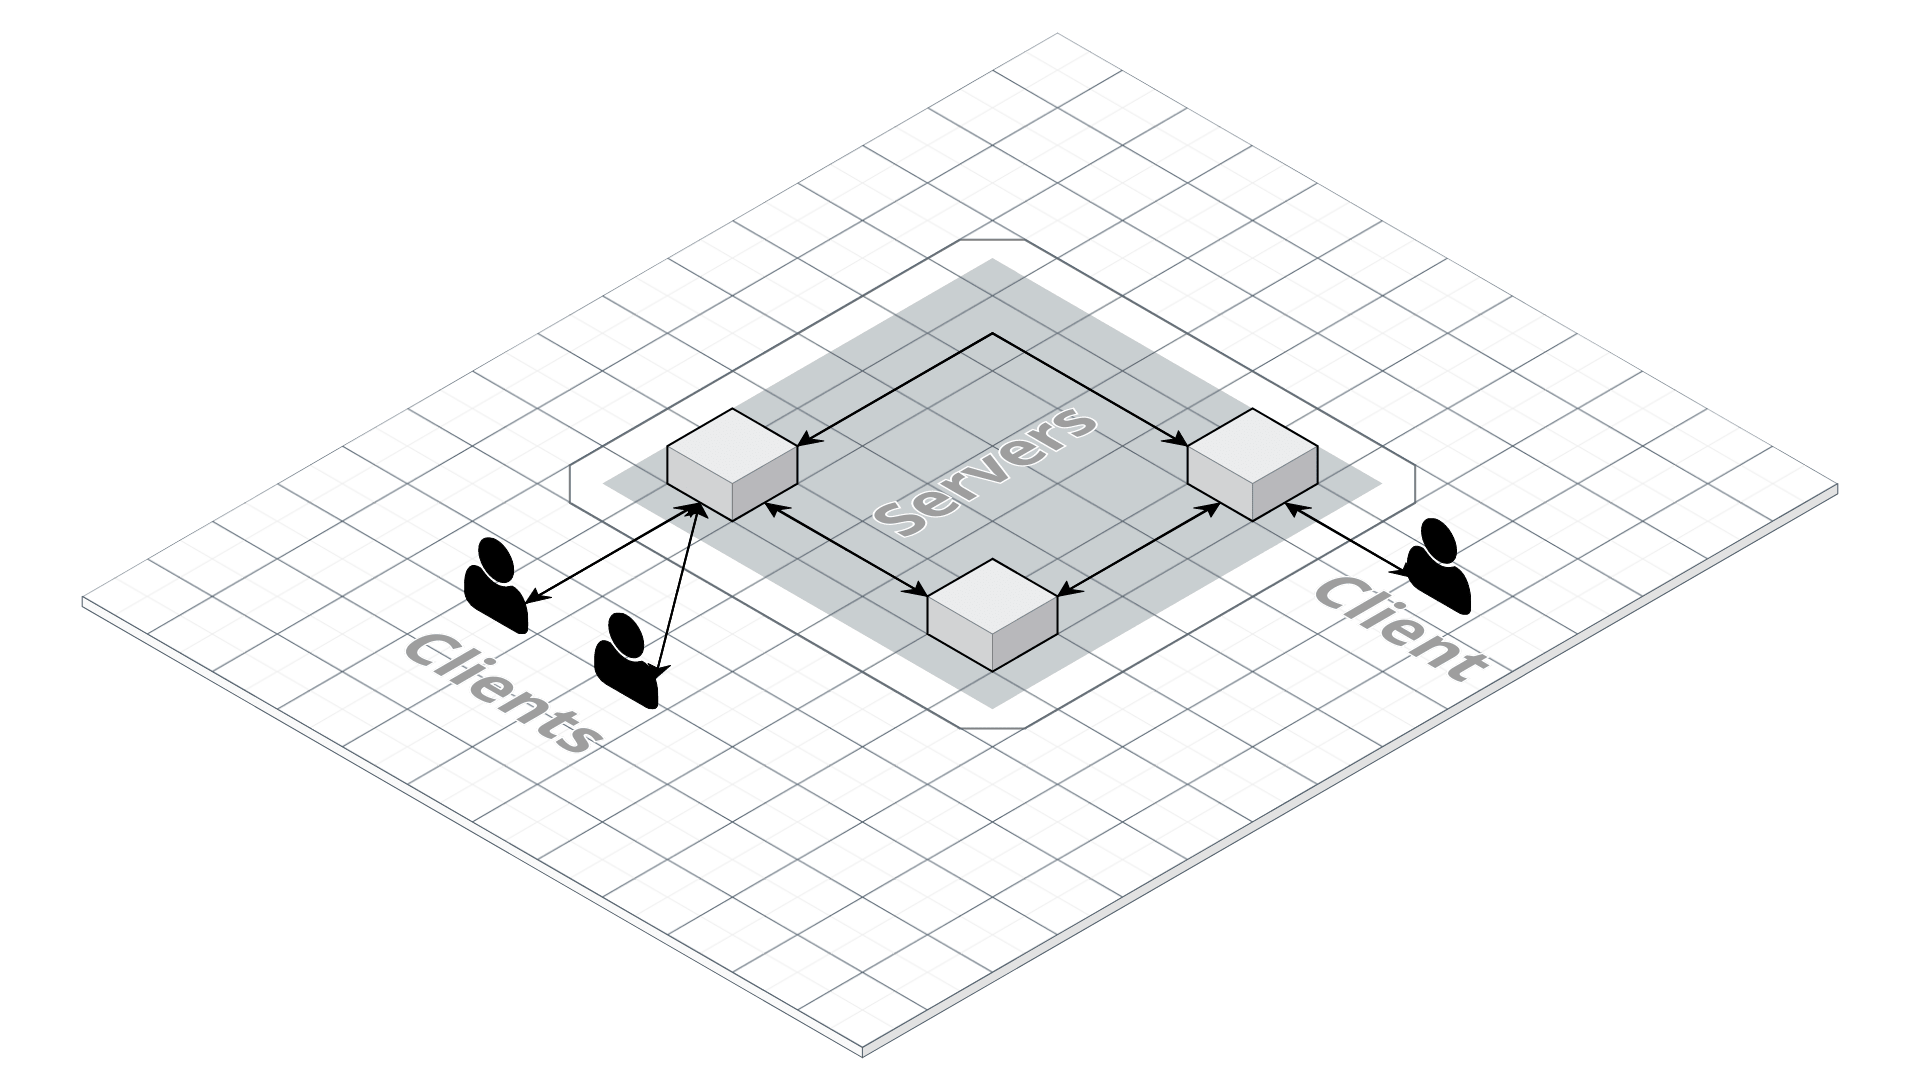
\includegraphics[width=\textwidth]{architecture.png}
    
    \caption{Architektur}
\end{figure}

\author{Matthias Vonend}
\subsection{Chatfunktionalität}\label{Chatfunktionalitaet}
Die Anwendung ist mit einem Thin Client aufgebaut. Damit ein Chat ablaufen kann, muss zunächst eine Verbindung zu einem Server aufgebaut werden.
Dazu wählt der Client zunächst einen zufälligen Server aus und versucht sich zu verbinden.
Wurde eine Verbindung erfolgreich aufgebaut, kann sich der Nutzer mit seinem Nutzernamen und seinem Passwort anmelden.
Sobald der Nutzer angemeldet ist, sendet der Server ihm alle benötigten Informationen inklusive der verpassten
Nachrichten zu. Der Server vergibt jeder eintreffenden Nachricht einen Timestamp, um zu dokumentieren, wann sie erstmalig eingetroffen ist.
Anhand des Timestamps werden die Nachrichten sortiert, damit der Client die korrekte Reihenfolge der Nachrichten darstellen kann.

Wenn ein Client eine Nachricht versenden möchte, wird das Nachrichtenpaket an die Node gesendet, mit der er verbunden ist.
Die Node kümmert sich im Hintergrund darum, die Nachricht an den Zielclient zuzustellen. 
Da alle Nachrichten aus Konsistenzgründen an alle Nodes verteilt werden müssen,
brauchen die Nodes keine Information über die Clients anderer Nodes. Im Falle einer solchen Anforderung
(z.\,B. Abfrage, ob ein anderer Nutzer aktiv ist) könnte ein Protokoll ähnlich zu Routing-Tabellen implementiert werden, um die zusätzliche Funktionalität bereitzustellen.
Empfängt eine Node eine Nachricht, egal ob von einem Client oder von einer anderen Node,
wird überprüft, ob die Nachricht für einen ihr bekannten Client bestimmt war. Wird ein Client gefunden, sendet die Node die Nachricht an den Zielclient.

\author{Jan Grübener, Troy Keßler, Patrick Mischka, Michael Angermeier}
\subsection{Clientfunktionalitäten}
Nach einer erfolgreichen Anmeldung kann der Nutzer zwischen verschiedenen Funktionen auswählen:
% \begin{itemize}
%     \item /help
%     \item /chats
%     \item /contacts
%     \item /createchat
%     \item /openchat
%     \item /exit
% \end{itemize}

\subsubsection*{/help:}
Diese Funktion gibt dem Nutzer einen Überblick über alle möglichen Funktionen, die er aufrufen kann.
Alle Funktionen sind kurz beschrieben, sodass der Nutzer einen Überblick über die Funktionen erhält.

\subsubsection*{/chats:}
Bei einem Aufruf dieser Funktion werden alle Chats, die für den Nutzer zugänglich sind, angezeigt.
%Dafür werden zunächst alle Chats durch die Methode getChats aus der API in einem Set aus Chats gespeichert.
Wenn Chats für den Nutzer verfügbar sind, werden diese in einer Übersicht mit Chatname und teilnehmenden Nutzen dargestellt.
Sind noch keine Chats vorhanden, wird darauf hingewiesen.

\subsubsection*{/contacts:}
Wird \textit{/contacts} aufgerufen, werden alle registrierten Nutzer angezeigt.

\subsubsection*{/createchat:}
Diese Funktion beginnt mit einer Aufforderung an den Nutzer, einen Chatnamen einzugeben.
Danach wird die Anzahl der Teilnehmer für den Chat erfragt, wobei mindestens ein Teilnehmer im Chat enthalten sein muss.
Im nächsten Schritt müssen alle Nutzernamen der Teilnehmer eingetragen werden. 
Jeder Nutzername wird auf seine Gültigkeit geprüft. Ist ein Nutzername ungültig, so wird darauf hingewiesen. 
%Hierfür wird jeder einzelne Nutzername überprüft und
% im Falle eines ungültigen Nutzernamens, wird der Nutzer durch eine Meldung darauf aufmerksam gemacht.
Wurden alle drei Attribute (Chatname, Teilnehmeranzahl, Nutzername der Teilnehmer) erfolgreich eingegeben,
wird ein neuer Chat erstellt.

\subsubsection*{/openchat:}
Will der Nutzer einen Chat öffnen, so muss er zuerst den Chatnamen eingeben. Ist der Chat vorhanden, so wird er geöffnet.
Kann der Chat nicht geöffnet werden, so wird eine Meldung für den Nutzer ausgegeben.
Am Anfang eines Chats wird immer darauf hingewiesen, wie der Chat
verlassen werden kann. Danach werden alle Nachrichten, die in diesem Chat bereits geschrieben wurden, geladen.
Anschließend kann der Nutzer Nachrichten versenden und empfangen.

\subsubsection*{/exit:}
Mithilfe dieser Funktion wird der Nutzer abgemeldet und Client beendet.

\author{Matthias Vonend, Aaron Schweig, Troy Keßler}
\subsection{Fehlerbehandlung}
Um Fehler und Datenverluste zu vermeiden, ist in dem Chatsystem sichergestellt, dass immer mindestens zwei Server (Nodes) \textbf{alle}
Informationen besitzen. So kann während eines Nodeausfalls gewährleistet werden, dass eine Andere alle Aufgaben übernehmen kann.

%Aus den Anforderungen geht hervor, dass es mindestens zwei Server geben muss, die sämtliche Informationen des
%Chatsystems besitzen müssen. Bricht eine Node zusammen, muss eine andere Node dessen Aufgabe übernehmen.
\subsubsection{Client}
Nachdem der Client eingeloggt ist, wartet er kontinuierlich auf neue Pakete vom Server. Stürzt eine Node ab, oder verliert der Client
die Netzwerkverbindung, so versucht er sich neu zu verbinden. Dabei wird eine neue, zufällige Node ausgewählt.
Kann der Client erfolgreich eine neue Verbindung aufbauen, meldet sich der Client mit den bestehenden Zugangsdaten an der Node an.
Ist diese nicht verfügbar, so wird so lange eine neue Node ausgewählt, bis eine Verbindung zustande kommt.
Im Regelfall findet der beschriebene Reconnect-Vorgang im Hintergrund statt.

\subsubsection{Server}
Serverseitig können verschiedene Fehler auftreten. Viele Fehler werden bereits durch das TCP-Protokoll und Java selbst verhindert 
(z.\,B. Mehrfachzustellung, fehlerhafte Übermittlung, \dots). Dennoch können grundsätzlich die folgenden Fehlerfälle eintreten:

\subsubsection*{Nachricht des Clients wird nicht korrekt gesendet/empfangen}
In diesem Fall muss der Server davon ausgehen, dass die Verbindung zusammengebrochen ist. Diese wird im Anschluss vom Server beendet
und wie bereits oben beschrieben versucht der Client erneut eine Verbindung aufzubauen.
Ist eine neue Verbindung wiederhergestellt, werden alle für den Client relevanten Nachrichten zu diesem übertragen 
und der Client muss fehlende Informationen erneut an den Server übertragen.

\subsubsection*{Nachrichten einer Nachbarnode werden nicht korrekt empfangen/gesendet}
Wie bereits im Kapitel \ref{Chatfunktionalitaet} beschrieben, tauschen Nodes alle Nachrichten untereinander aus. Innerhalb des Chatsystems können mehrere
Netzwerktopologien realisiert werden. Die ausfallsicherste Variante stellt dabei eine Mesh-Struktur dar. 
Diese ermöglicht es, auch bei einem Ausfall mehrerer Nodes, alle Nachrichten mit allen bekannten Nachbarnodes zu synchronisieren. Netzwerkpartitionierungen sind damit
deutlich schwerer zu erreichen und auch mehrerer Nodeausfälle können mithilfe der Mesh-Topologie kompensiert werden. Ebenfalls wird durch die Wahl der
Write-All-Available Replikationsstrategie sichergestellt, dass alle bekannten Nachbarnodes komplett synchronisiert sind.
\\
Tritt ein Fehler in der Verbindung zwischen verschiedenen Nodes auf, so muss die Node ähnlich wie bei einem Fehler im Client davon ausgehen, 
dass die Verbindung zusammengebrochen ist. Allerdings sind die Nodes hier selbst für eine Fehlerbehandlung zuständig und versucht eine neue
Verbindung aufzubauen. Um sicherzustellen, dass keine konkurrierenden Schreibzugriffe auf den OutputStream stattfinden,
werden Nachrichten in einer Queue aufbewahrt bevor sie an andere Nodes übertragen werden.
\\
Werden die Nodes getrennt sind die Clients immer noch in der Lage Nachrichten an ihre jeweiligen Nodes zu schicken.
Sobald eine Verbindung wieder aufgebaut wurde, synchronisieren sich die Nodes, um einen vollständigen Informationsstand wiederherzustellen.
Sind keine Nachrichten zu senden, hat die Node keine Möglichkeit festzustellen, ob eine Verbindung noch existiert. 
Zu diesem Zweck existiert ein Heartbeat, der periodisch die Nachbarnodes anpingt und so prüft, ob die Verbindung noch existiert.
Jede Node prüft dabei, 
ob sie alle Informationen des empfangenen Warehouses bereits besitzt und fügt geg. neue Informationen hinzu. 
Sofern die Node neue Informationen erhalten hat, broadcastet diese ihren neuen Stand an alle benachbarten Nodes,
um diese auch auf den neuesten Stand zu bringen.



